与任何加速器架构一样,预测FPGA何时是加速器的正确选择,何时需要替代方案,通常取决于对架构、应用程序特征和系统瓶颈的了解。本节描述要考虑的一些特征。\par

\hspace*{\fill} \par %插入空行
\textbf{海量任务}

大多数现代的计算机加速器,想要获得良好的性能需要大量的工作。单个数据元素计算单个结果,对于加速器是没有加速效果的。这与FPGA一样,了解了FPGA编译器利用了流水线并行性,这一点就更加明显了。算法的流水化实现有很多阶段,通常是上千个甚至更多,每个阶段在任何时钟周期内都应该有不同的工作。如果没有足够的工作在占用流水线的大部分阶段,那么执行效率就会很低。\par

有多种方法可以在FPGA上生成工作来填充流水线阶段,我们将在接下来的章节中介绍这些方法。\par

\hspace*{\fill} \par %插入空行
\textbf{自定义操作或操作宽度}

FPGA最初用来执行整数和位操作,并作为逻辑粘合剂,可以使其他芯片的接口工作。虽然FPGA已经发展成为计算功能强大的设备,已不仅仅是粘合逻辑解决方案,但在位操作、自定义数据宽度或类型上的整数数学操作,以及对包头信息中的任意位字段的操作方面仍然非常高效。\par

本章末尾描述的FPGA的细粒度架构意味着可以有效地实现新的任意数据类型。例如,如果我们需要33位整数乘法器或129位加法器,FPGA可以以很高的效率提供这些操作。由于这种灵活性,FPGA通常用于快速发展的领域,例如:机器学习,其中数据宽度和操作的变化速度比内置在专用集成电路中要快。\par

\hspace*{\fill} \par %插入空行
\textbf{标量数据流}

从图17-4可以明显看出,FPGA空间流水线的一个重要方面是,操作之间的中间数据不仅停留在芯片上(没有存储到外部内存),而且每个管道阶段之间的中间数据都有专用的存储寄存器。FPGA的并行性来自于流水线,同时执行许多操作,每个操作在流水线的不同阶段。这与向量体系结构不同,在向量体系结构中,多个计算作为共享向量指令的路径执行。\par

空间流水线中并行性的标量性质,对于许多应用程序都很重要,因为即使在跨工作单元的紧密数据依赖情况下仍然适用。可以在不损失性能的情况下处理这些数据依赖关系,我们将在本章后面讨论循环具有依赖关系时对此进行讨论。空间流水线对于不能破坏跨工作单元(如工作项)的数据依赖,并且可以进行细粒度通信。其他加速器的许多优化技术都侧重于打破这些依赖关系,或者通过子工作组等特性在可控范围内管理通信。相反,FPGA可以很好地处理依赖与通信,应该考虑在存在这种模式的算法中使用FPGA。\par

\begin{tcolorbox}[colback=blue!5!white,colframe=blue!75!black, title=循环不是罪!]
对于数据流体系结构的一个常见误解是,具有固定或动态迭代计数的循环会导致糟糕的数据流性能,因为它们不是简单的前馈流水。至少对于Intel DPC++和FPGA工具链来说,这不正确。相反,循环迭代是在流水线中产生高占用率的一种好方法,而编译器是以重叠的方式执行多个循环迭代构建的。循环提供了一种简单的机制来保持流水线忙于工作!
\end{tcolorbox}

\hspace*{\fill} \par %插入空行
\textbf{低延迟和富连接}

利用设备上丰富的输入和输出收发器的FPGA的更传统的使用同样适用于使用DPC++的开发人员。例如,如图17-6所示,一些FPGA加速卡具有网络接口,可以将数据直接流进设备,进行处理后将结果直接流回网络。当需要最小化处理延迟、通过操作系统网络栈进行的处理太慢或需要卸载时,通常会寻求这种系统。\par

\hspace*{\fill} \par %插入空行
图17-6 低延迟I/O流:FPGA连接网络数据和计算
\begin{center}
	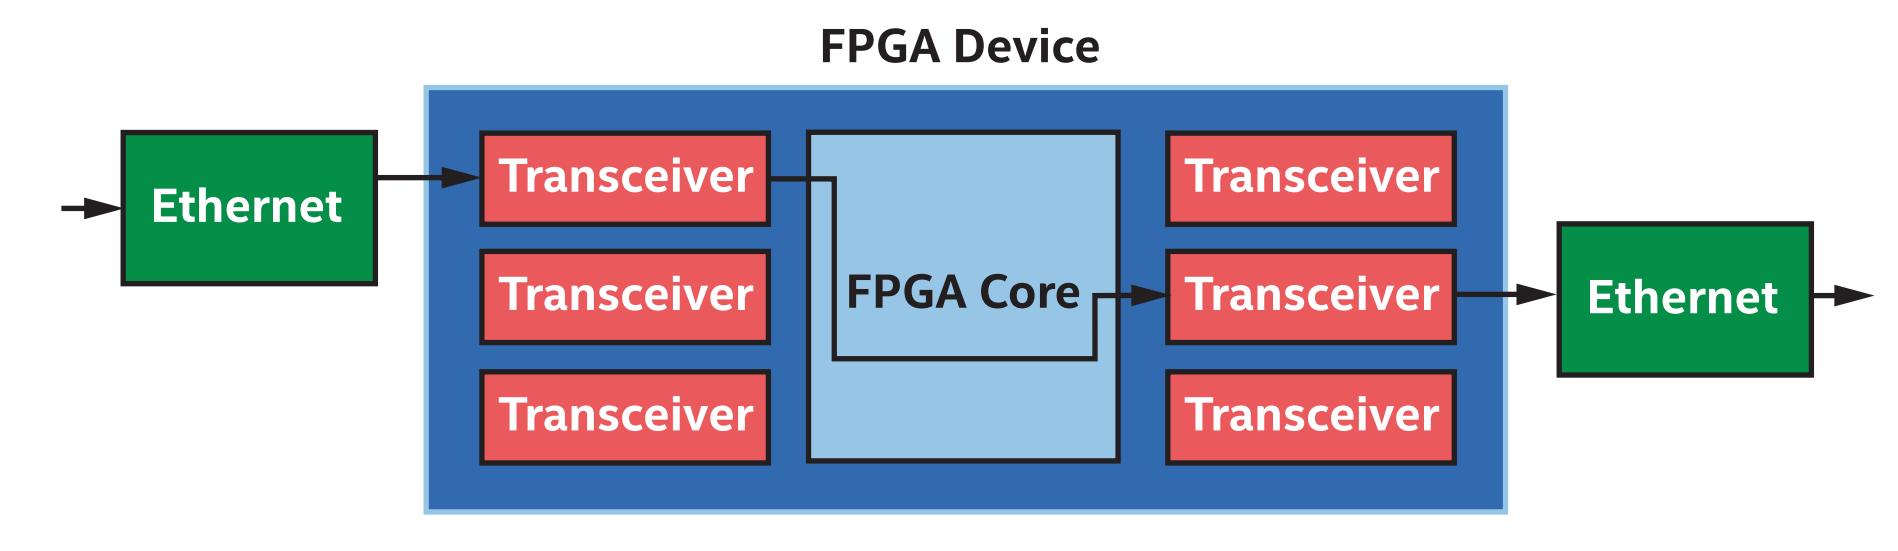
\includegraphics[width=1.0\textwidth]{content/chapter-17/images/7}
\end{center}

当考虑通过FPGA收发器直接输入/输出时,机会有很多,但选择确实取决于加速器上可用的东西。由于依赖于特定的加速卡和各种场景,除了在下一节中描述管道语言构造外,本章不深入研究这些应用程序。相反,我们应该阅读与特定加速卡相关的供应商文档,或者搜索与特定接口需求相匹配的加速卡。\par

\hspace*{\fill} \par %插入空行
\textbf{定制的内存系统}

FPGA上的存储系统,私有存储器或工作组本地存储器,是由片上存储器构建。每个内存系统都是为使用它的算法或内核的特定部分定制构建的。FPGA具有显著的片上存储器带宽,并且结合形成定制存储器,可以在具有非典型存储器访问模式和结构的应用程序上表现得很好。图17-7显示了在FPGA上实现内存系统时,编译器可以执行的一些优化。\par

\hspace*{\fill} \par %插入空行
图17-7 FPGA存储系统是由编译器为特定代码定制的
\begin{center}
	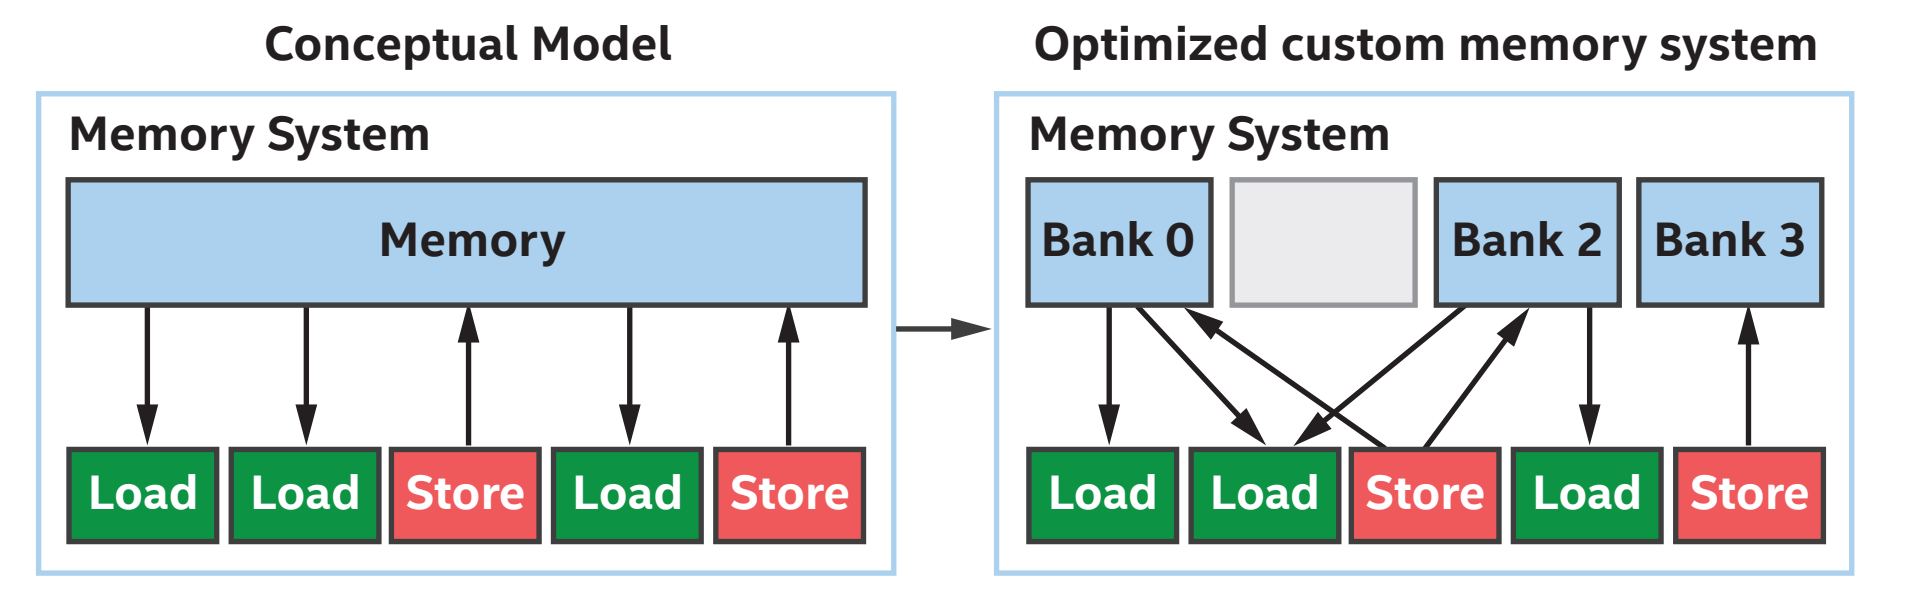
\includegraphics[width=1.0\textwidth]{content/chapter-17/images/8}
\end{center}

其他架构(如GPU)具有固定的内存结构,这很容易使有经验的开发人员理解,但在许多情况下很难进行优化。例如,其他加速器的许多优化都集中在内存模式修改,以避免内存块冲突。如果算法能够从自定义的内存结构中获益,比如每个内存块的访问端口数量不同,或者内存块数量异常,那么FPGA就有直接的优势。从概念上讲,两者的区别在于编写代码高效地使用固定的内存系统(大多数其他加速器),而让编译器定制内存系统,来提升特定代码的性能(FPGA)。\par



























